% !TEX root = ../thesis.tex

\chapter{Design \& Implementation}
\label{cha:design_implementation}
% Θα πρότεινα αυτό το κεφάλαιο να είναι Design and Implementation για τη
% βασική προσέγγιση. Πρώτα ο αλγόριθμος που θα μπορεί να αναφερθεί σε πράγματα
% που ήδη έχεις καλύψει από το κεφ. 2 [π.χ. τι είναι ETag; πώς χρησιμοποιώ ένα API
% στο οποίο κάθε αρχείο έχει το δικό του URL κλπ], και μετά προχωράς στην
% περιγραφή του βασικού Pythonικού σκελετού.

\section{Syncing Algorithm}
  \subsection{Known algorithms}
    The process of synchronising two filesystem trees (henceforth called ``A'' and ``B'') can be complex to perform correctly, if some needed information is missing. Differences in files can be detected by comparing their hash digests, which is often used as an ETag. While this is the most secure and reliable way to detect changes, computing the hash digest of a file, especially when using a cryptographically secure function) is a computationally expensive procedure that takes significant time for large files. The last modification time is a fast and cheap way to detect file changes, but since it is a property that can be manipulated by software, improper or malicious manipulation can result in failure to detect changes.\\

     First of all, history data for those two trees are very important, as illustrated in the following example. There are generally three cases when synchronising two trees:
    \begin{enumerate}
      \item File exists on both and is identical
      \item File exists on both and is different
      \item File exists on A but not on B (or vice-versa)
    \end{enumerate}
    Case 1 is easily handled, since there is no action to be taken. Without history information, the other two cases would require user input in order to be handled correctly. In case 2, the files should be merged, but cannot be done automatically - and asking regular users how to merge files is undesirable. In case 3, the file might be a newly created, or a recently deleted one and should be copied to tree B or deleted from A, respectively. While the safe choice is to assume the file is new and copy it to tree B, it is often \textbf{not} the right thing to do. It is therefore clear that without file history data the syncing algorithm makes wrong assumtions and fails to handle correctly the most common cases.\\

    With file history present in the form of metadata, a more proper synchronisation is achievable. By checking what changes occured and when between the times $T_1$ and $T_2$, it is possible to determine the action that should be taken, based on table \ref{table:simple-sync-actions}:\\

    \begin{table}[H]
      \centering
      \begin{tabular}{|l|l|l|}
        \hline \textbf{File replica A} & \textbf{File replica B} & \textbf{Action} \\ \hline \hline
         No Change & No Change & No Action \\ \hline
         Created (ETag = J) & Created (Etag = J) & No Action \\ \hline
         Created (ETag = J) & Created (Etag = K) & \emph{Merge$^*$} \\ \hline
         Deleted & Deleted & No Action \\ \hline
         Deleted & No Change & Delete B \\ \hline
         Modified & No Change & Update B \\ \hline
         Modified (ETag = J) & Modified (ETag = K) & \emph{Merge$^*$} \\ \hline
      \end{tabular}
      \caption{Syncing actions based on file states}
      \label{table:simple-sync-actions}
    \end{table}

    [*] In this table, \emph{Merge} refers to a situation where files A and B become identical. One way this can be achieved is by generating diffs and patching the files, requiring user input if a conflict arises - this is the way most Version Control Systems (VCS), like git and Mercurial, work. A different way, that requires no immediate user interaction is to accept one file version (e.g. File A) and propagating its changes to all other trees, while also renaming the conflicting files, so the conflicts can be manually merged later.

    For any given time, detecting what happened between the times $T_1$ and $T_2$, is straightforward, and described in \ref{table:time-change-detection}:\\

    \begin{table}[H]
      \centering
      \begin{tabular}{|l|l|l|}
        \hline \textbf{Time $T_1$} & \textbf{Time $T_2$} & \textbf{Change}\\ \hline \hline
         Does not Exist & Exists & Created \\ \hline
         Exists & Does not Exist & Deleted \\ \hline
         Exists (ETag = J) & Exists (Etag = J) & No Change \\ \hline
         Exists (Etag = J) & Exists (Etag = K) & Modified \\ \hline
      \end{tabular}
    \caption{File change detection between two points in time}
    \label{table:time-change-detection}
    \end{table}

    While this algorithm is significantly better than the previous one, it still has limitations, the most important of which is the failure to detect renames. This can become possible by comparing file digests, but doing so for all files in a directory or for very large files is computationally expensive and slows down the sync process. An even harder problem is the detection of a file that has been renamed and modified, hence having a different hash digest than the original one, a case most syncing algorithms fail to handle efficiently.\\

  \subsection{Proposed Algorithm}
    \label{ssec:3step_algorithm}
    At this point we propose a new sychronisation algorithm, one which is efficient, fast and reliable. We assume a service that uses a central metadata server, which maintains information about each version of an uploaded object. We also assume the usage of a local state database, henceforth called \textbf{StateDB}, which locally stores the metadata of all files in the local directory, as they were during the last synchronisation with the server. More specifically, a path hash is used as a file identifier, and other important metadata saved are the file name (``path''), the inode, last modification time (``modtime''), and the file's hash digest(``Etag''). Now the problem of reconcilation between the local directory replicas (``Local'') and the remote server replicas (``Remote'') can be now handled in three steps.

    \subsubsection{Step 1: Detect updates from Local Directory}
      For each file in the local directory, the necessary action can be derived from the decision tree in Figure \ref{fig:step1}.

      \begin{figure}[H]
        \centering
        \begin{tikzpicture}[thick]
        \newdimen\nodeDist
        \nodeDist=30mm

          \node [state] (A) {phash exists in StateDB?};
          \path (A) ++(-155:1.6\nodeDist) node [state] (B) {Local modtime == StateDB modtime?};
          \path (A) ++(-25:1.6\nodeDist) node [state] (C) {inode exists in StateDB?};

          \path (B) ++(-125:\nodeDist) node [block] (B-1) {No local change};
          \path (B) ++(-55:\nodeDist) node [state] (B-2) {File exists on Remote?};
          \path (B-2) ++(-125:\nodeDist) node [state] (B-2-1) {StateDB ETag == Remote Etag?};
          \path (B-2) ++(-55:\nodeDist) node [block] (B-2-2) {Local modified};
          \path (B-2-1) ++(-125:\nodeDist) node [block] (B-2-1-1) {Local modified};
          \path (B-2-1) ++(-55:\nodeDist) node [block] (B-2-1-2) {Conflict};

          \path (C) ++(-125:\nodeDist) node [block] (C-1) {Renamed};
          \path (C) ++(-55:\nodeDist) node [state] (C-2) {File exists on remote?};
          \path (C-2) ++(-125:\nodeDist) node [block] (C-2-1) {Conflict};
          \path (C-2) ++(-55:\nodeDist) node [block] (C-2-2) {New local file};


          \draw (A) -- (B) node [left,pos=0.4] {yes};
          \draw (A) -- (C) node [right,pos=0.4] {no};
          \draw (B) -- (B-1) node [left,pos=0.5] {yes};
          \draw (B) -- (B-2) node [right,pos=0.5] {no};
          \draw (B-2) -- (B-2-1) node [left,pos=0.5] {yes};
          \draw (B-2) -- (B-2-2) node [right,pos=0.5] {no};
          \draw (B-2-1) -- (B-2-1-1) node [left,pos=0.5] {yes};
          \draw (B-2-1) -- (B-2-1-2) node [right,pos=0.5] {no};
          \draw (C) -- (C-1) node [left,pos=0.5] {yes};
          \draw (C) -- (C-2) node [right,pos=0.5] {no};
          \draw (C-2) -- (C-2-1) node [left,pos=0.5] {yes};
          \draw (C-2) -- (C-2-2) node [right,pos=0.5] {no};
        \end{tikzpicture}
        \caption{Decision tree for local directory files}
        \label{fig:step1}
      \end{figure}

    \subsubsection{Step 2: Detect updates from StateDB}
      For each entries in the StateDB, the necessary action can be derived from the decision tree in Figure \ref{fig:step2}.

      \begin{figure}[H]
        \centering
        \begin{tikzpicture}[scale=0.92, thick, every node/.style={transform shape}]
        \newdimen\nodeDist
        \nodeDist=30mm

          \node [state] (S) {File exists on local/remote?};
          \path (S) ++(-160:2.4\nodeDist) node [blstate] (A) {Local exists, Remote exists};
          \path (A) ++(0:1.5\nodeDist) node [blstate] (C) {Local doesn't exist, Remote exists};
          \path (C) ++(0:1.5\nodeDist) node [blstate] (B) {Local doesn't exist, Remote doesn't exist};
          \path (B) ++(0:1.5\nodeDist) node [blstate] (D) {Local exists, \hspace{1em} Remote doesn't exist};
          \path (A) ++(-90:0.7\nodeDist) node [block] (AA) {No change};
          \path (B) ++(-90:0.7\nodeDist) node [block] (BB) {Deleted};
          \path (C) ++(-90:0.7\nodeDist) node [state] (CC) {inode exists in StateDB?};
          \path (CC) ++(-120:\nodeDist) node [block] (CC-1) {Renamed / Deleted};
          \path (CC) ++(-60:\nodeDist) node [state] (CC-2) {Remote ETag == StateDB Etag?};
          \path (CC-2) ++(-120:\nodeDist) node [block] (CC-2-1) {Deleted};
          \path (CC-2) ++(-60:\nodeDist) node [block] (CC-2-2) {Remote modified};
          \path (D) ++(-90:0.7\nodeDist) node [state] (DD) {Local modtime == StateDB modtime?};
          \path (DD) ++(-120:\nodeDist) node [block] (DD-1) {Deleted};
          \path (DD) ++(-60:\nodeDist) node [block] (DD-2) {Local modified};


          \draw (S) -- (A);
          \draw (S) -- (B);
          \draw (S) -- (C);
          \draw (S) -- (D);
          \draw (A) -- (AA);
          \draw (B) -- (BB);
          \draw (C) -- (CC);
          \draw (D) -- (DD);
          \draw (CC) -- (CC-1) node [left,pos=0.5] {yes};
          \draw (CC) -- (CC-2) node [right,pos=0.5] {no};
          \draw (CC-2) -- (CC-2-1) node [left,pos=0.5] {yes};
          \draw (CC-2) -- (CC-2-2) node [right,pos=0.5] {no};
          \draw (DD) -- (DD-1) node [left,pos=0.5] {yes};
          \draw (DD) -- (DD-2) node [right,pos=0.5] {no};
        \end{tikzpicture}
        \caption{Decision tree for StateDB entries}
        \label{fig:step2}
      \end{figure}

    \subsubsection{Step 3: Detect updates from Remote Server}
      In accordance to the previous steps, the necessary action for each file in the remote server can be derived from the decision tree in Figure \ref{fig:step3}

      \begin{figure}[H]
        \centering
        \begin{tikzpicture}[thick]
        \newdimen\nodeDist
        \nodeDist=30mm

          \node [state] (A) {phash exists in StateDB?};
          \path (A) ++(-125:\nodeDist) node [state] (B) {Remote ETag == StateDB ETag?};
          \path (A) ++(-55:\nodeDist) node [block] (C) {New remote file};

          \path (B) ++(-125:\nodeDist) node [block] (B-1) {No remote changes};
          \path (B) ++(-55:\nodeDist) node [state] (B-2) {Local modtime == StateDB modtime?};
          \path (B-2) ++(-125:\nodeDist) node [block] (B-2-1) {Remote modified};
          \path (B-2) ++(-55:\nodeDist) node [block] (B-2-2) {Conflict};

          \draw (A) -- (B) node [left,pos=0.4] {yes};
          \draw (A) -- (C) node [right,pos=0.4] {no};
          \draw (B) -- (B-1) node [left,pos=0.5] {yes};
          \draw (B) -- (B-2) node [right,pos=0.5] {no};
          \draw (B-2) -- (B-2-1) node [left,pos=0.5] {yes};
          \draw (B-2) -- (B-2-2) node [right,pos=0.5] {no};
        \end{tikzpicture}
        \caption{Decision tree for remote server files}
        \label{fig:step3}
      \end{figure}

    \subsubsection{Notes on the syncing algorithm}
      \begin{itemize}
        \item This algorithm offers a resilient synchronisation process. Since it completely processes each file, there is no problem if a partial sync is made because of an interruption.
        \item For update detection between Local and StateDB, we use modtime, since it is faster. For update detection between StateDB and Remote, we use the ETag, since it is the most reliable way and is readily available without hashing the file - it is stored in both cases and available with only a lookup.
        \item When the file is updated on Local but deleted on Remote, we decide to upload the modified file again, since it is the safe option.
        \item If conflict is detected, that means that the both the Local file and the Remote one have been updated since the last sync was completed. In that case we propose to rename the local one to ``<filename>-conflicting\_copy.<extension>'' and download the remote one. Filenames ending in ``-conflicting\_copy'' are excluded from Step 1 of the syncing algorithm.
        \item In step 2, figure \ref{fig:step2}, ``\textbf{No change}'' means that there is no action to be taken at this point. There might be changes in the files, but they will be handled by steps 1 and 3.
        \item In step 2, figure \ref{fig:step2}, ``\textbf{Renamed / Deleted}'' means that we are unsure whether the file has been renamed or deleted. If a FileID info (a string, created once at the creation time of the file that changes over the file's lifetime) is supported and available from the remote server (as ownCloud does), it should be easy to decide which of the two possible actions should be taken.
        Without this information, we suggest an alternative way to handle this case, without performing a costly reverse-inode lookup. When a file falls in this category during step 2, we add its inode to a \emph{delete\_set}. During step 1, for each file in the local directory, we discard its inode from the \emph{delete\_set}, if it exists. When the algorithm reaches step 2 again, all remaining files in the \emph{delete\_set} should be deleted.
      \end{itemize}


\section{Basic Classes / API}
  \subsection{FileStat}
    \begin{figure}[!htpb]
      \centering
      
\includegraphics{Images/FileStat.eps}
      \caption{FileStat UML class description}
      \label{fig:filestat_uml}
    \end{figure}
    FileStat is the core class used in this framework to represent a file object's status. The StateDB stores entries with this format and the other classes and methods use instances of this class to refer to files.
    \begin{itemize}
      \item \textbf{phash (int)}: The hash digest of the relative path string. Currently uses the xxh64 hash function, for the reasons explained below. It is the main identifier of a file.
      \item \textbf{path (str)}: The path of the file, relative to the root synchronisation directory.
      \item \textbf{inode (int)}: The index node of the file on the file system. Used mostly for rename detection.
      \item \textbf{modtime (int)}: The last modification time of a file. It is stored in the POSIX format (UNIX epoch), for accurate and timezone-independent representation.
      \item \textbf{type (int)}: The type of the file. Added for possible future features, depending on the file type (document, image, binary object, etc).\\
      Currently only the following two values are used: \{0 = Regular file, 1 = Directory\}.
      \item \textbf{etag (str)}: The ETag of the file. Current implementation uses the SHA-256 digest of the file. Hashing is not done locally, but uses the hashed value produced and stored on the server.
    \end{itemize}

    \subsubsection{Path hash algorithm selection}
      We needed the path hash (phash) algorithm to be consistent and provide hash values that are both collision resistant and large enough (in bits) as to provide a large enough set of permissible outputs and prevent collisions occuring from the birthday problem. Generating the hash of a path occurs often, so a fast hash function is preferable to a cryptographic but slower one. The most notable hash functions that fit this description were MurmurHash 3 and xxHash\cite{xxhash}, and we decided to use the latter, because it was faster and a better Python library was available to use in the framework.

  \subsection{StateDB}
    \begin{figure}[!htpb]
      \centering
      \begin{subfigure}{0.45\textwidth}
        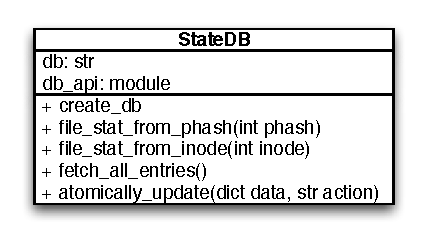
\includegraphics[width=\textwidth]{Images/StateDB.eps}
        \caption{StateDB UML class description}
        \label{fig:statedb_uml}
      \end{subfigure}
      \begin{subfigure}{0.45\textwidth}
        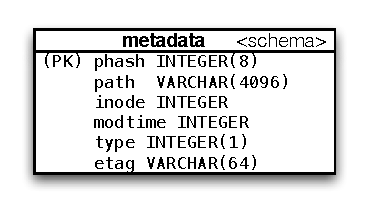
\includegraphics[width=\textwidth]{Images/StateDB_schema.eps}
        \caption{StateDB schema}
        \label{fig:statedb_schema}
      \end{subfigure}
      \caption{StateDB}
      \label{fig:statedb}
    \end{figure}
    StateDB is the class that manages the state database, which stores the metadata of the files during the time each was last synchronised. The current implementation uses the SQLite library with the sqlite3 module, because it is reliable, fast and lightweight, properties that are important for the framework. SQLite also offers a \emph{row\_factory} attribute, enabling us to return the results as FileStat objects, instead of rows (tuples). Nevertheless, the class has been designed to be easily used with a different database engine, and just needs any python module that conforms to the Python Database API Specification v2.0 (PEP-249)\cite{pep-249}. The schema used for the database, as seen in figure \ref{fig:statedb_schema}, has the same attributes as the FileStat object. A brief explanation of StateDB attributes and methods follows:

    \begin{itemize}
      \item \textbf{db}: The full path of the database file (sqlite3 uses files to store the database)
      \item \textbf{db\_api}: Any PEP 249-compliant DB API module.\\
      \item \textbf{create\_db}: Creates the metadata database, if it doesn't already exist, using the schema in figure \ref{fig:statedb_schema}.
      \item \textbf{file\_stat\_from\_phash}: Returns a FileStat object for the given \emph{phash} if it exists, else returns \emph{None}.
      \item \textbf{file\_stat\_from\_inode}: Returns a FileStat object for the given \emph{inode} if it exists, else returns \emph{None}.
      \item \textbf{fetch\_all\_entries}: Returns all entries in the StateDB as FileStat objects. Uses a generator that fetches 1000 entries at a time, in order to reduce memory footprint in cases of large databases.
      \item \textbf{atomically\_update}: Atomically updates the StateDB, using the \emph{data} and \emph{action} specified in the arguments. For sqlite, we use a 2-phase commit mechanism, copying the database to a temporary location, updating the copy and then moving the updated copy back to the original's location, in order to emulate an atomic commit.
    \end{itemize}

  \subsection{LocalDirectory}
    \begin{figure}[!htpb]
      \centering
      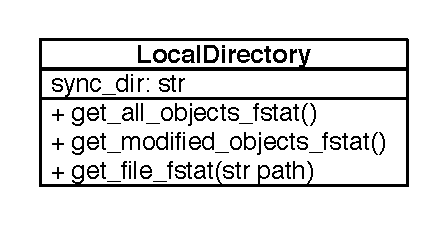
\includegraphics{Images/LocalDir.eps}
      \caption{LocalDirectory UML class description}
      \label{fig:localdir_uml}
    \end{figure}
    LocalDirectory is the base Class that represents the local sync directory. A brief explanation of LocalDirectory attributes and methods follows:
    \begin{itemize}
      \item \textbf{sync\_dir}: The full path of the root directory to be synchronised.\\

      \item \textbf{get\_all\_objects\_fstat}: Returns all local files' metadata as FileStat objects. Uses a generator to reduce memory footprint.
      \item \textbf{get\_modified\_objects\_fstat}: Return file metadata only for the files that were modified since the last sync. On the base implementation it returns all files in the directory, as if \textbf{get\_all\_objects\_fstat()} was called.
      \item \textbf{get\_file\_fstat}: Returns the FileStat object for the file \emph{path} if it exists, else returns \emph{None}.
    \end{itemize}

  \subsection{CloudClient}
    \label{ssec:cloudclient}
    \begin{figure}[!htpb]
      \centering
      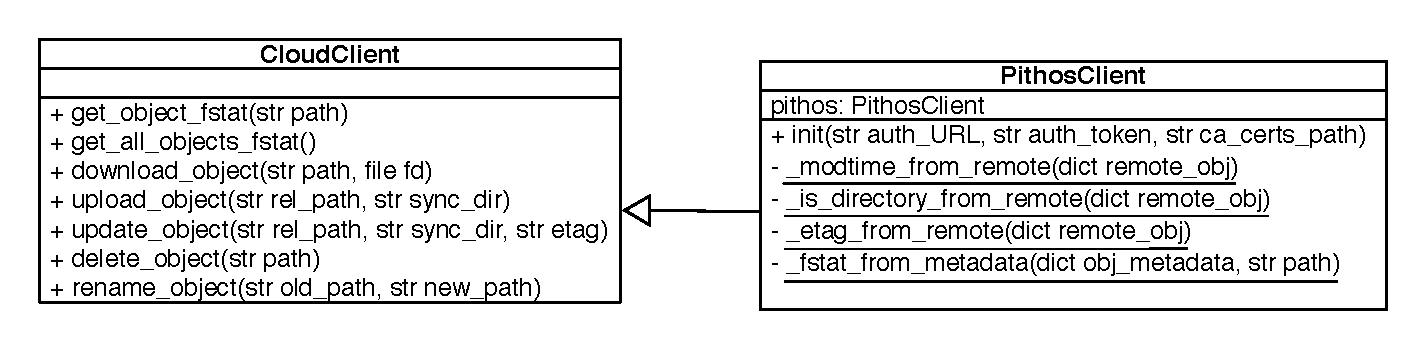
\includegraphics[width=1.1\textwidth]{Images/CloudClient.eps}
      \caption{CloudClient - PithosClient UML class description}
      \label{fig:cloud_uml}
    \end{figure}
    CloudClient is the base class for representing an Object Storage service client. None of the methods shown in \ref{fig:cloud_uml} are implemented on the base class and just serve as an API designation. Derived classes should implement those methods and extend the class with their own, where necessary. In this dissertation, we show an example subclass with Pithos (File/Object Storage) services of synnefo, as used in the \textasciitilde okeanos IaaS. A brief explanation of CloudClient and PithosClient attributes and methods follows:
    \subsubsection{CloudClient}
      \begin{itemize}
        \item \textbf{get\_object\_fstat}: Returns the metadata of the file \emph{path} stored on the remote server as a FileStat object.
        \item \textbf{get\_all\_objects\_fstat}: Returns the metadata of all files stored on the remote server as FileStat objects.
        \item \textbf{download\_object}: Downloads the file \emph{path}, saving its contents to the file desciptor \emph{fd}.
        \item \textbf{upload\_object}: Uploads the local file from \emph{rel\_path} to the remote server. Fails if the file already exists on the server.
        \item \textbf{update\_object}: Updates the the remote server replica with the changes in local file \emph{rel\_path}. Checks for race condition, updating only if the \emph{etag} matches the one stored in StateDB, else fails.
        \item \textbf{delete\_object}: Deletes the remote server file \emph{path}.
        \item \textbf{rename\_object}: Renames the remote server file \emph{old\_path} to \emph{new\_path}. Fails if \emph{new\_path} exists on the server.
      \end{itemize}
    \subsubsection{PithosClient}
      \begin{itemize}
        \item \textbf{pithos}: An authenticated client which calls the Pithos API functions of the service, when needed.\\
        \item \textbf{init}: Uses \emph{auth\_URL} and \emph{auth\_token} to authenticate a pithos client with Astakos (the Identity Management Service), then prepares it for use.
        \item \textbf{\_modtime\_from\_remote}: Static method that returns the modtime in POSIX format (UNIX epoch timestamp), given the remote file metadata response \emph{remote\_obj}. Used for disambiguation, since the json responses of pithos service follow two different formats.
        \item \textbf{\_is\_directory\_from\_remote}: Static method that returns \emph{True} if the object is a folder, given the remote object metadata response \emph{remote\_obj}. Used for disambiguation.
        \item \textbf{\_etag\_from\_remote}: Static method that returns the etag, given the remote file metadata response \emph{remote\_obj}. Used for disambiguation.
        \item \textbf{\_fstat\_from\_metadata}: Returns the FileStat object of a file, given its metadata response \emph{remote\_obj}.
      \end{itemize}

  \subsection{Syncer}
    \begin{figure}[!htpb]
      \centering
      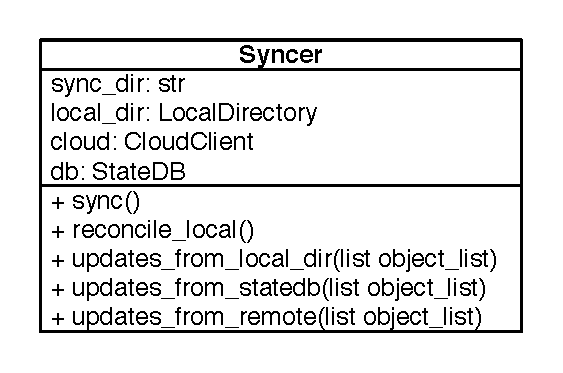
\includegraphics{Images/Syncer.eps}
      \caption{Syncer UML class description}
      \label{fig:syncer_uml}
    \end{figure}
    Syncer is the class that manages the synchronisation process between a local directory and a remote object storage service. A brief explanation of Syncer attributes and methods follows:
    \begin{itemize}
      \item \textbf{sync\_dir}: The full path of the root directory to be synchronised.
      \item \textbf{local\_dir}: The LocalDirectory object to be used during sync.
      \item \textbf{cloud}: The authenticated CloudClient object to be used during sync.
      \item \textbf{db}: The StateDB object to be used during sync.\\

      \item \textbf{sync}: Executes a full local-remote sync, using the 3-step algorithm described in section \ref{ssec:3step_algorithm}.
      \item \textbf{reconcile\_local}: Checks all files in the local directory for updates and performs the necessary actions for their synchronisation, as described in figure \ref{fig:step1}.
      \item \textbf{updates\_from\_local\_dir}: Checks all files in the \emph{object\_list} for updates and performs the necessary actions for their synchronisation, as described in figure \ref{fig:step1}.
      \item \textbf{updates\_from\_statedb}: Checks all files in the \emph{object\_list} for updates and performs the necessary actions for their synchronisation, as described in figure \ref{fig:step2}. \emph{object\_list} is generated by fetching all entries in the StateDB.
      \item \textbf{updates\_from\_remote}: Checks all files in the \emph{object\_list} for updates and performs the necessary actions for their synchronisation, as described in figure \ref{fig:step3}. \emph{object\_list} is generated by fetching all remote files' metadata.
    \end{itemize}